\documentclass[12pt,a4paper,final]{report}			%definire grandezza testo, foglio e tipo di testo.
\usepackage[headheight=20mm, width=150mm,top=23mm,bottom=23mm,left=25mm,right=25mm]{geometry}
\usepackage{pdf14}
\usepackage[utf8]{inputenc}			%definisce la codifica dei caratteri
\usepackage[italian]{babel}				%definisce il pacchetto della lingua
\usepackage{amsmath}						%contiene molti utili strumenti per la scrittura matematica
\usepackage{amsfonts}
\usepackage{amssymb}
\usepackage{makeidx}
\linespread{1.2}
\usepackage{units} 					%unita di misura
\usepackage{subcaption}  		%per le figure
\usepackage{subcaption}		%DON'T KNOW. INVESTIGATE
\usepackage{siunitx} 				%unita SI
\usepackage{mathrsfs}			%per usare cose tipo \mathscr{}
\usepackage{physics}				%contiene molta notazione utile; lo uso in particolare per \bra e \ket
\usepackage{cite}
\usepackage{comment}
\usepackage{caption}
\usepackage[font=small,labelfont=bf]{caption}		% serve per ridurre la dimensione delle captions
\usepackage[final]{pdfpages}		%per poter includere pdf
\usepackage[a-1a]{pdfx}
\usepackage[pdfa]{hyperref}
%\pdfminorversion=4

\title{Riassunto di tesi}

\begin{document}
\begin{center}
	\LARGE \textbf{Stima delle proprietà di sistemi ottici nelle microonde tramite l'utilizzo di reti neurali}
	%\textbf{Stima delle proprietà di sistemi ottici nelle microonde tramite l'utilizzo di reti neurali.}
\end{center}
\begin{center}
	\normalsize \textit{Eleonora Gatti}
\end{center}

\vspace{5mm}


%CMB
L’obiettivo di questo lavoro di tesi è quello di costruire una rete neurale che sia in grado di prevedere i parametri che caratterizzano la risposta angolare di un ricevitore, quali ellitticità, full width half maximum e cross-polarizzazione, in funzione di una posizione sulla superficie focale di uno strumento. In questa tesi ho inoltre confrontato le prestazioni di reti neurali con metodi tradizionali basati sull'interpolazione di tali parametri.

%DIAGRAMMA RADIAZIONE

\begin{comment}
La \textbf{CMB}, Cosmic Microwave Background, \`e la radiazione a microonde di fondo cosmico che permea l’intero Universo, originatasi dal disaccoppiamento tra materia e radiazione, avvenuto circa 380\,000 anni dopo il Big Bang. Lo studio della CMB è estremamente importante perché consente di studiare le condizioni in cui l'Universo si è formato, andando a caratterizzare i suoi parametri fisici in tempi molto prossimi al Big Bang (fino a $10^{-30}\,\text{s}$).
\end{comment}

Negli esperimenti di fondo cosmico, e più in generale in qualsiasi esperimento di radioastronomia, è molto importante non solo misurare il segnale, ma anche ricostruire accuratamente la sua direzione di provenienza. La risposta di un sistema ottico si quantifica solitamente tramite il cosiddetto \textbf{diagramma di radiazione}, una funzione matematica $\gamma$ che associa a una direzione sulla sfera celeste $(\theta, \phi)$ l'efficienza nel catturare la radiazione: per un sistema ideale $\gamma(\theta, \phi) = 1$ se l'efficienza è massima, $\gamma(\theta, \phi) = 0$ se lo strumento è cieco lungo tale direzione. Il diagramma di radiazione mostra tipicamente la presenza di un \textit{main beam}, un lobo principale nella posizione del polo nord ($\theta = 0$), nel quale è contenuta la maggior parte della radiazione.

%PARAMETRI

A partire dal diagramma di radiazione si definiscono alcuni parametri che lo descrivono. I parametri analizzati in questo lavoro di tesi sono: la \textbf{Full Width Half Maximum} (FWHM) del main beam che è la larghezza angolare a metà della sua altezza; l'\textbf{ellitticità}, che misura il livello di simmetria intorno all'asse del main beam; la componente \textbf{co-polare massima} che quantifica la potenza ricevuta lungo la direzione di polarizzazione della sorgente; la componente \textbf{cross-polare massima} che quantifica la potenza ricevuta lungo la direzione perpendicolare a quella di polarizzazione.


%SIMULAZIONI
I software per la simulazione di sistemi ottici nelle microonde simulano la propagazione della radiazione in un sistema ottico, consentendo di stimare $\gamma(\theta, \phi)$.
Ad ogni posizione sulla superficie focale corrisponde uno specifico diagramma di radiazione e ogni simulazione permette di valutare un solo diagramma di radiazione (ad una simulazione è quindi associata una particolare posizione). Per caratterizzare un sistema ottico è necessario effettuare numerose simulazioni, pari almeno al numero di detector dello strumento studiato. 
Tuttavia, tali simulazioni sono molto dispendiose in termini di tempo e per sistemi ottici complessi, con migliaia di detector sulla superficie focale, risulta impossibile una simulazione completa dell'ottica.
Allo stesso tempo per raggiungere sensibilità strumentali elevate che consentano di rivelare segnali molto deboli, come ad esempio la CMB\footnote{La CMB, Cosmic Microwave Background, \`e la radiazione a microonde di fondo cosmico che permea l’intero Universo, originatasi dal disaccoppiamento tra materia e radiazione, avvenuto circa 380\,000 anni dopo il Big Bang. Lo studio della CMB è estremamente importante perché consente di studiare le condizioni in cui l'Universo si è formato, andando a caratterizzare i suoi parametri fisici in tempi molto prossimi al Big Bang (fino a $10^{-30}\,\text{s}$).}, è fondamentale avere a disposizione vasti piani focali che permettano di utilizzare un elevato numero di rivelatori.

\`E quindi forte la necessità di trovare una via alternativa che consenta di stimare i parametri che descrivono il beam in una qualsiasi posizione.

%OBIETTIVO
In questa tesi ho voluto verificare se una rete neurale riuscisse a predire i parametri di interesse più efficacemente rispetto ad un'interpolazione. In particolare l'obiettivo è stato quello di stabilire un criterio per discriminare la bontà dei diversi metodi di stima dei parametri del diagramma di radiazione, e di individuare metodi più rapidi per la stima di $\gamma(\theta, \phi)$, o almeno dei suoi parametri più rappresentativi.

%DATASET

Quale caso d'analisi, ho scelto l'ottica di STRIP, telescopio a doppio riflettore dell'esperimento LSPE per l'osservazione della polarizzazione della CMB sulle grandi scale angolari. L'ottica di STRIP è stata simulata tramite il software GRASP, che ha fornito i parametri del beam elencati sopra (FWHM, ellitticità, \ldots) per differenti posizioni sulla superficie focale del telescopio.
Tali posizioni sono espresse come coordinate $(x,y,z)$ in uno spazio cartesiano e definiscono una griglia $13\text{x}13$ lungo le componenti $x$ e $y$. 

A partire dal dataset ottenuto tramite le simulazioni in GRASP ho creato due subsets per effettuare rispettivamete l'interpolazione/training della rete e la verifica della bontà dei dati stimati.

%PROCEDURA
Per stimare le proprietà di un diagramma di radiazione attraverso strumenti classici di interpolazione ho utilizzato due metodi: \texttt{interp2d} del modulo \texttt{scipy.interpolate}, basato su un'interpolazione lineare tra punti adiacenti, e \texttt{curve\_fit} del modulo \texttt{scipy.optimize}, con cui ho fatto un fit ai minimi quadrati tra i dati e un paraboloide. Dal momento che \texttt{interp2d} ha mostrato problemi, soprattutto per i punti ai bordi del piano focale, nel resto della mia analisi ho trascurato di includerlo nei confronti.


Parallelamente ho stimato il valore dei parametri attraverso reti neurali di tipo \textit{feed forward} e \textit{fully connected}.
Ho creato 6 diverse architetture di rete che variano per funzione di attivazione (\textit{Tanh} o \textit{Sigmoid}) e numero di hidden layers (1, 2, 3). 
I risultati che ho ottenuto mostrano che le reti neurali hanno prestazioni migliori rispetto ai metodi di interpolazione, o al più equiparabili.
Il grafico sotto riportato mostra la distribuzione degli errori relativa ad uno dei parametri elencati sopra (ellitticità), confrontata tra diversi tipi di reti neurali (in blu) e il caso migliore dell'interpolazione (in arancione).


Questa tesi rappresenta un punto di partenza per ulteriori studi futuri che permetteranno una simulazione dei parametri del diagramma di radiazione per strumenti che includano un elevato numero di ricevitori, come per esempio LiteBIRD ($\sim10^3$ rivelatori), e per i quali è impossibile effettuare una simulazione dell'intera ottica attraverso i software di simulazione.
Sarà estremamente interessante rieffettuare l'analisi proposta in questa tesi utilizzando un dataset più ampio o ancora analizzare i dati relativi ad uno strumento con una superficie focale diversa da quella di STRIP.


\begin{comment}
Quanto hai scritto qui va bene, ma in un riassunto di tesi questo livello di dettaglio è solitamente più del richiesto. Dì semplicemente che i tuoi risultati mostrano che le reti neurali hanno prestazioni migliori rispetto ai metodi di interpolazione, e dì che il grafico sotto mostra la distribuzione degli errori relativa ad uno dei parametri elencati sopra (ellitticità), confrontata tra diversi tipi di reti neurali e il caso migliore dell'interpolazione.

Ho suddiviso dataset iniziale il \texttt{training\_set} (75\%) e \texttt{validation\_set} (25\%). Ho inoltre normalizzato i dati di output (ovveo i valori dei parametri del beam) per facilitare la convergenza della rete. Ho effettuato il training della rete su 30000 epoche rimescolando i dati del \texttt{training\_set}  e del \texttt{validation\_set} ogni 5000 epoche. 
Ho poi riassunto risultati ottenuti attraverso dei \textit{violin plots} i quali permettono di visualizzare la densità di probabilità di ottenere un determinato valore dell’errore e di confrontare, in un unico grafico, i risultati relativi all'interpolazione e quelli relativi alle varie architetture di rete. Tanto più è piccata la curva per valori bassi dell’errore, quanto più il risultato è buono.
\`E qui riportato il violin plot relativo all'ellitticità per la quale si può osservare che alcune architetture di rete (per esempio Tanh\_2L) forniscono risultati apprezzabilmente migliori rispetto a quelli ottenuti con l’interpolazione.

Confronto dell'errore tra dato stimato e dato esatto relativo all'ellitticità. Il grafico mostra il confronto tra i risultati ottenuti tramite i diversi tipi di rete neurale e tramite interpolazione.
\end{comment}

\vspace{1cm}
\begin{figure}[!ht]
    \centering
    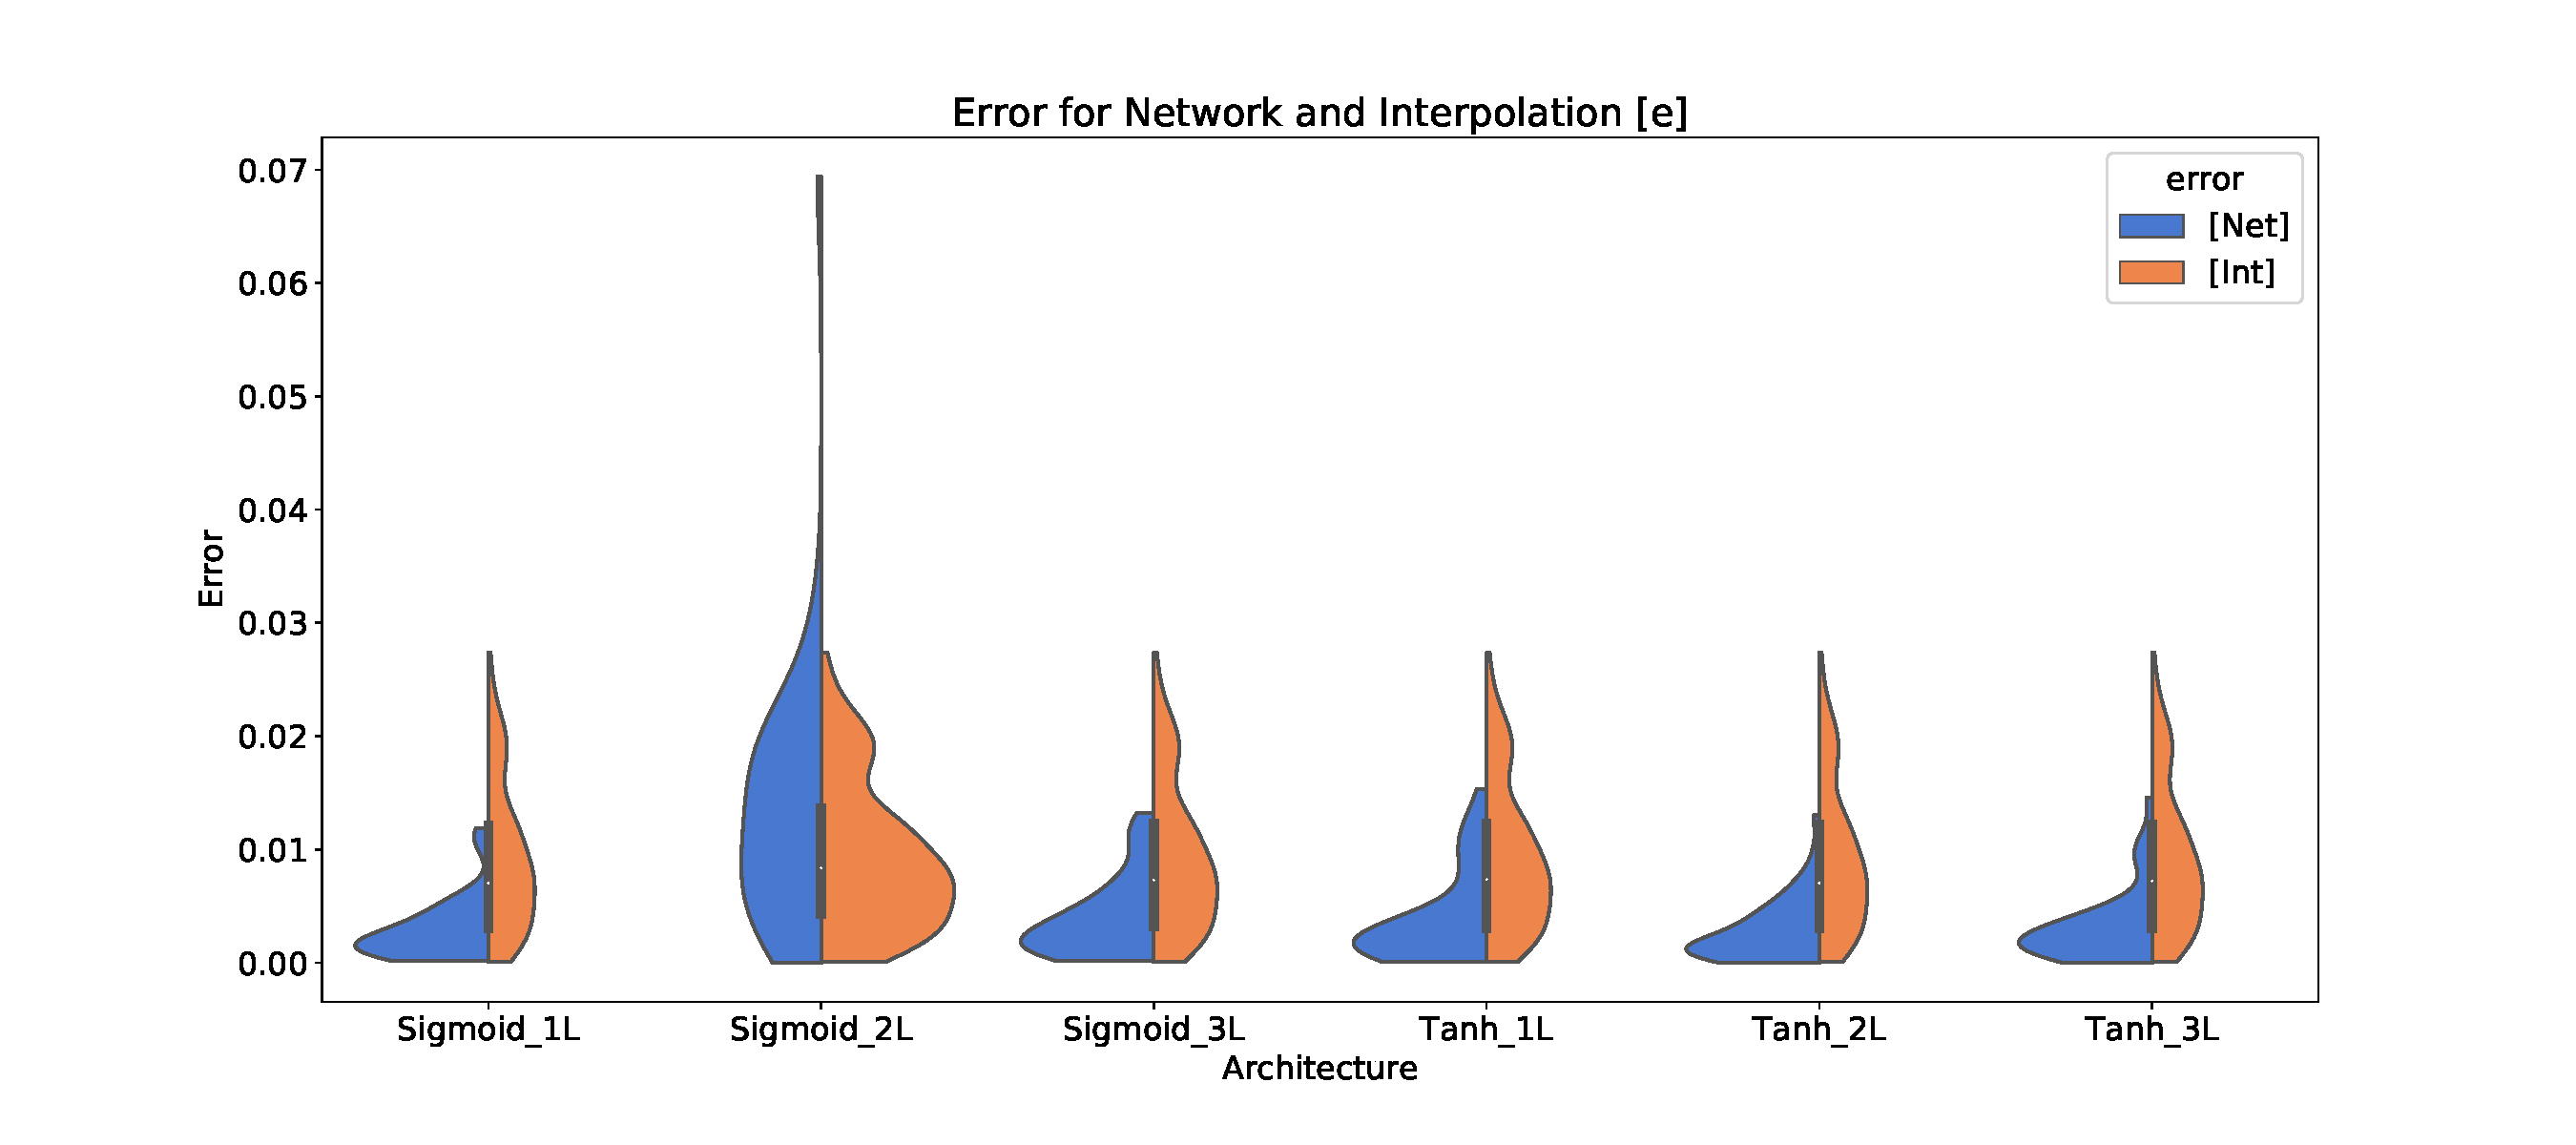
\includegraphics[width=\linewidth]{../figures/violin_plot_e.pdf}
\end{figure}


\end{document}
